\documentclass{article}
\usepackage{amssymb,amsfonts,amsmath,calc,tikz,geometry}
\usepackage{color}   %May be necessary if you want to color links
\usepackage{hyperref}
\usepackage{amsthm}
\hypersetup{
    colorlinks=false, %set true if you want colored links
    linktoc=all,     %set to all if you want both sections and subsections linked
    linkcolor=black,  %choose some color if you want links to stand out
}
\geometry{margin=1in}
\newcommand{\N}{\mathbb{N}}
\newcommand{\Z}{\mathbb{Z}}
\newcommand{\Q}{\mathbb{Q}}
\newcommand{\R}{\mathbb{R}}
\newcommand{\Omicron}{O}
\theoremstyle{plain}
\newtheorem{theorem}{Theorem}[section]
\newtheorem{lemma}[theorem]{Lemma}
\newtheorem{proposition}[theorem]{Proposition}
\newtheorem{corollary}[theorem]{Corollary}
\newtheorem{definition}{Definition}[section]
\newtheorem{remark}{Remark}[section]
\newcommand{\bigslant}[2]
{{\raisebox{.2em}{$#1$}\left/\raisebox{-.2em}{$#2$}\right.}}
\title{\textbf{Set Theory I}}
\author{Yeheli Fomberg}
\date{}

\usepackage{amsmath}
\begin{document}
\maketitle
\newpage
\tableofcontents
\newpage
\section{Permutations}
	A permutation $\sigma$ is a bijection from a set $S$ onto iteself.
	\begin{center}
		$\sigma=$
			$\begin{pmatrix}
				1 & 2 & 3 & 4 & 5\\
				2 & 5 & 4 & 3 & 1\\
			\end{pmatrix}$
		=$(3 \ 4)(1 \ 2 \ 5)$
	\end{center}
	\begin{enumerate}
		\item A cycle of one element is call a \textbf{fixed point}
		\item A permutation without fixed points is called a 
		\textbf{derangement}
		\item A permutation that's an orbit of 2 elements is called a 
		\textbf{transposition}
	\end{enumerate}
	
	\subsection{The symmetric group}
	A symmetric group defined over a set is the group whose elements are 
	all the permutation over the set, and whose group operation is the 
	composition of functions.
	\begin{remark}
	A group is an algebraic structure with the following 
	characteristics:
	\end{remark}
	\begin{itemize}
		\item \text{Associativity}
		\item \text{An idenentity permutation exists}
		\item \text{Every element has an inverse}
	\end{itemize}
		
	\newpage
	\section{Hall's theorem}
	\begin{definition}
		In a bipartite graph $G=(X,Y,E)$ the \textbf{neighborhood} of a subset
		$X'$ of $X$ denoted $N_G(X')$ is the set of all the vertices in 
		$Y$ that share an edge with some vertex from $X'$.
	\end{definition}
	\begin{theorem}
	\textbf{Hall's theorem} - In a finite bipartite graph $G(X,Y,E)$ 
	a perfect matching exists if and only if for any subset $W$ of $X$ 
	exists an injection from $W$ to $N_G(W)$.
	\end{theorem}
	\noindent \underline{$(\Leftarrow)$} \\
	Suppose we have an $X$ perfect matching. Since for any given $W$ 
	all vertices in $W$ have a distinct matching vertex in $Y$,
	we get that the matching function is an injection from $W$ to $N_G(W)$.\\
	\\ \underline{$(\Rightarrow)$} \\
	We will prove by contradiction. Assume an $X$-perfect matching doesn't 
	exist, we can denote the maximal matching $M$, and the sets of vertices 
	in $X,Y$ that appear in $M$ as $S,T$.
	Since an $X$-perfect matching doesn't exist we get
	$X\setminus S \neq \emptyset$, 
	so we can choose a vertex $u_0 \in X \setminus S$ and consider all 
	alternating paths of the form $P=(u_0,v_1,v_2,\ldots)$ such that 
	odd edges are not in $M$ and even edges are in $M$.
	Denote:
	\begin{align*}
		A &= \{u \mid u\in P \land u\in X\} \\
		B &= \{v \mid v\in P \land v\in Y\}
	\end{align*}
	We know every vertex in $B$ is matched by $M$ to a vertex in $A$ 
	because otherwise we could create a bigger matching by toggling 
	whether each of the edges belong to $M$ or not.
	\[
		\Rightarrow |B| \le |A \setminus \{u_0\}| \Rightarrow |B| < |A|
	\]
	But also for any vertex $a\in A$, all of its neighbors are in $B$ which
	implies
	\[
		N_g(A) \le B
	\]
	We can also show that an alternating path to $b$ exists either by removing 
	the matched edge $ab$ from the alternating path to $a$, or by adding 
	the unmatched edge $ab$ to the alternating path to $a$.
	\begin{align*}
		&\Rightarrow B = N_g(A) \\ 
		&\Rightarrow |N_g(A)|<|A|
	\end{align*}
	That's a contradiction so an $X$-perfect matching must exist.
		
	\newpage
	\section{Cantor's theorem}
	\begin{theorem}
	Cantor's theorem - for any set $A$
	\[
		|A| < |P(A)|
	\]
	\end{theorem}
	\noindent We can define $f \colon A \to P(A)$ as such:
	\[
		f(a) = \{a\}
	\]
	This is clearly an injection so we get:
	\[
		 |A| \le |P(A)|
	\]
	Assume $|A|=|P(A)|$. 
	That means there's a bijection $g \colon A \to P(A)$. Consider the 
	following set:
	\[
		D = \{ a : a \notin g(a)\}
	\]
	Since $g$ is a bijection exists $b\in A$ such that $f(b)=D$. Now  
	consider the different cases:
	\[
		\begin{cases}
		b\in D, & b\notin g(b)=D \implies \text{contradiction} \\
		b\notin D=g(b), & b\in D \implies \text{contradiction}
		\end{cases}
	\]
	Therefore $|A| \neq |P(A)|$ which implise $|A| < |P(A)|$
		
		
\newpage
	\section{Equivalence Relations}
	An equivalence relation is a binary relation, or a set of ordered pairs 
	that is:
	\begin{itemize}
	\item Reflexive
	\item Symmetric
	\item Transitive
	\end{itemize}
	
	\subsection{Some Terminology}
		Suppose we have an equivalnce relation $R$ on a set $X$.
		\begin{definition}
			An \textbf{equivalence class} denoted $[a]_R$ is defined
			as:
			\[
				\{ b \in X \mid bRa = 1 \}
			\]
		\end{definition}
		\begin{definition}
			A \textbf{quotient set} denoted $\bigslant{X}{R}$ is defined as
			such:
			\[
				\{ [a]_R \mid a \in X \}
			\]
		\end{definition}
		\begin{definition}
			A \textbf{projection} of $R$ is a function 
			$\pi \colon X \to \bigslant{X}{R}$ such that:
			\[
				\pi(x) = [x]_R
			\]
		\end{definition}
		\begin{definition}
			A \textbf{cut} of $X$ is a set with only one element of each 
			equivalence class.
		\end{definition}
	\noindent Equivalence relations can be defined by their quotient set.
	Thus they can also be defined by a function or a partition.
	The numbers of partitions of a set $|X|=n$ are known as Bell's numbers 
	and can be calculated recursivly as such:
	\[
		B_{n+1} = \sum_{k=0}^{n}{n \choose k} B_k
	\]
	Think why.
	
\newpage
\section{Kőnig's Theorem}
	\begin{theorem}
	Kőnig's Theorem - For an index set $I$, if for all $i \in I$ and 
	$\kappa_i, \lambda_i$ we know that $\kappa_i < \lambda_i$ then:
	\[
		\sum_{i\in I}{\kappa_i} < \prod_{i\in I}{\lambda_i}
	\]
	\end{theorem}
	\noindent We will show this by proving that for any:
	\[
		f \colon \sum_{i\in I}{B_i} \to \prod_{i\in I}{C_i} 
		\quad\text{such that}\quad
		|B_i| = \kappa_i \text{ and } |C_i|=\lambda_i
	\]
	That $f$ is not surjective. Define the function $f_i$ as such:
	\begin{align*}
		f_i \colon B_i \to C_i \\
		f_i(x) = f(x)_i
	\end{align*}
	For all $i\in I$ we have $|B_i|<|C_i|$ which implies that for all 
	$i\in I$ that $f_i$ is not surjective. Therefore for all $i\in I$ exist 
	$c_i \in C_i \setminus \mathrm{Im}(f_i)$. Consider the vector: 
	\[
		\hat{c} = \ \langle c_i \mid i\in I \rangle
	\]
	If $\hat{c} \in \mathrm{Im} f$ then exist $i \in I$ and 
	$b \in B_i$ such that $f(b) = \hat{c}$. This implies that $f(b)_i=c_i$
	so $f_i(b)=c_i$ but since $c_i \in C_i\setminus \mathrm{Im}f_i$
	we get a contradiction. Therefore: 
	\[
		\left| \sum_{i\in I}{B_i} \right| < \left|\prod_{i\in I}{C_i}\right| 
		\implies
		\sum_{i\in I}{\kappa_i} < \prod_{i\in I}{\lambda_i}
	\]

\newpage

\section{Partial Orders}
\begin{definition}
	A \textbf{Weak/Non-Strict} Partial Order is a homogeneous relation 
	$\le$ on a set $P$ that is:
\end{definition}
\begin{itemize}
	\item Reflexive
	\item Antisymmetric \footnote[1]{$a\le b \land b\le a \Rightarrow a=b$}
	\item Transitive
	\end{itemize}
\begin{definition}
	A \textbf{Strong/Strict Partial} Order is a homogeneous relation 
	$<$ on a set $P$ that is:
\end{definition}
\begin{itemize}
\item Irreflexive
\item Asymmetric\footnote[2]{$a<b \Rightarrow \lnot b<a$}
\item Transitive
\end{itemize}
\begin{remark}
	We have that $< \bigcup \le_{Id} = \le$
\end{remark}

\section{Partially Ordered Sets}
\begin{definition}
	A \textbf{Partially Ordered Set} also known as a poset is an ordered
	pair of a set and a partial order $(A,\le)$.
\end{definition}
\begin{definition}
	Two elements $a, b \in A$ are called \textbf{comparable} if and
	only if $a \le b$ or $b \le a$. If two elements are incomparable 
	they are called \textbf{linearly independent}.
\end{definition}
\begin{definition}
A \textbf{linear/total order} is a partial order under which every pair of 
elements is comparable. All ordered subsets which are called \textbf{chains} 
are linearly independent of each other.
\end{definition}
\subsection{Extrema}
\begin{definition}
A \textbf{greatest element} is an element that's comparable and greater 
than all other elements
\end{definition}
\begin{definition}
A \textbf{maximal element} is an element that doesn't have a greater element 
than him.
\end{definition}
\begin{definition}
An \textbf{upper bound} in $A$ of $B\subseteq A$ is an element $a\in A$ such
that for every $b \in B$ we have $b \le a$. 
Similarly, a \textbf{lower bound} in 
$A$ of $B\subseteq A$ is an element $a \in A$ such that for every $b \in B$ 
we have $a \le b$.
\end{definition}

\subsubsection{About Lattices}
\begin{definition}
A partially ordered set $A$ is a \textbf{lattice} if and only if for
every $S\subseteq A$ with two elements, $\sup S$, $\inf S$ exist.
\end{definition}
    
\newpage
\section{Cardinals}
Cardinal numbers are the ``numbers'' we use to represent the size of 
sets. We denote the cardinality of $\N$ as $\aleph_0$, and the cardinality
of $\R$ as $\aleph$. To get good intuition for cardinals I suggest trying 
to prove the following:
\begin{enumerate}
    \item $|\N| < |\R|$
    \item $\aleph_{0}$ = 
    $\aleph_{0} + n = \aleph_0 \times n=\aleph_0\times\aleph_0=|\Z|=|\Q|$
    \item $\aleph = 2^{\aleph_0} = |(0,1)^{\aleph_0}| = \aleph\times\aleph_0 
    = \aleph\times\aleph = |(0,1)| = |[0,1]|$
    \item A plane can't be covered by $\aleph_0$ lines.
    \item Let A be an infinte set, $\exists S\subseteq A : |S|=\aleph_0$
    \item $\aleph = |P(\N)|= |P(\Q)|$
    \item let A = \{The set of all finite subsets of $\N$\} prove 
    $|A|=\aleph_0$
    \item $\aleph^\aleph_0=\aleph$
    \item $|\R^\R|=|P(\R)|=2^\aleph$
    \item $|$The disjoint union of $\N$ sets of size $\N|$= $\aleph_0$
    \item $\aleph_0^{\aleph_0} =\aleph$
    \item $|$The set of all invertible functions $\R\rightarrow\R|$ 
    = $2^\aleph$
    \item $|A|=|$The set of all algebraic numbers$|=\aleph_0$
    \item $|B|=|\R\setminus A|=|$The set of all transcedental number$|=\aleph$
    \item $|$All subsets of $\R$ with cardinality $\aleph/\aleph_0|$
    \item Let $\aleph_0$ people with a natural number of hats on their head 
    guess how many hats they have. How many options are there, given only 
    a finite number of people guessed right/wrong?
    
\end{enumerate}


\newpage
\section{Schröder–Bernstein Theorem}
\begin{theorem}
The \textbf{Schröder–Bernstein Theorem} states that:
\[
	|A| \le |B| \land |B| \le |A| \iff |A| = |B|
\]
\end{theorem}
\noindent The left direction is trivial, to prove the other direction
suppose we have two injective functions:
\begin{align*}
f \colon A \rightarrow B \\
g \colon B \rightarrow A
\end{align*}
Without loss of generality, assume $A$, $B$ are disjoint.
\footnote{Why can we do this?}
Using the partially defined functions $f^{-1}$, $g^{-1}$ we can construct 
a sequence for every element of $A \cup B$ in the following way:
\[
	\ldots \to f^{-1}g^{-1}(a) \to g^{-1}(a) 
	\to a \to f(a) \to g(f(a)) \to \ldots
\]
This sequence can keep going forever to the right, but to the left it 
may stop eventually since the inverse functions are partial
\footnote{We'll call those who stop from the left on an element 
of $A$ $A$-stops and the rest $B$-stops - even though they may not 
always stop!}. 
We can see that every element in $A \cup B$ has a sequence and that 
if an element appears in two sequnces they'll be identical since 
they're injective and by our construction. Thus those sequences form 
a partition of $A \cup B$ so it is sufficient to create bijections 
for all partitions. Our bijection will be:
\[
    h(x) = \begin{cases}
        f(x), & \text{for } x\in A\text{ in an $A$-stop}\\
        g^{-1}(x), & \text{for } x\in A\text{ in a $B$-stop}\\
        f^{-1}(x), & \text{for } x\in B\text{ in an $A$-stop}\\
        g(x), & \text{for } x\in B\text{ in a $B$-stop}\\
        \end{cases}
\]
It's not hard to show that this function is well defined and a bijection
for each sequence. Therefore $h$ is a bijection from $|A|$ to $|B|$ as wanted.

\newpage

\section{Homomorphism and Isomorphosm of Ordered Sets}
\subsection{Homomorphisms}
Let $(X,\le_1) , (Y,\le_2)$ be partially ordered sets.
\begin{definition}
A function between posets $F$ is a \textbf{homomorphism} if and only if
for every $x_1,x_2 \in X$ 
\[
	x_1 \le_1 x_2 \Rightarrow F(x_1) \le_2 F(x_2)
\]
\end{definition}
\subsection{Isomorphisms}
\begin{definition}
A function between posets $F$ is an \textbf{isomorphism} if and only if
it is a bijection and for every $x_1,x_2 \in X$ 
\[
	x_1 \le_1 x_2 \Rightarrow F(x_1) \le_2 F(x_2)
\]
\end{definition}
\noindent An isomorphism is reflexive, symmetric and transitive so it is 
an equivalnce relation. If $F$ is an isomorphism and the orders are 
total orders then $F^{-1}$ is also an isomorphism.
\subsection{Lexicographic Order}
Also known as a ``dictonary order'' is an order such that:
\[
	(x_1,y_1) \le (x_2,y_2) 
	\iff 
	x_1 <_{x} x_2 \lor (x_1=x_2 \land y_1 \le_{y} y_2)
\]
It is also a partial order on $X\times Y$.

\newpage
\section{Zorn's Lemma}
\begin{lemma}
\textbf{Zorn's lemma} - Let $F$ be a non-empty poset.
If for every chain
\footnote{a totally ordered subset} 
in $F$ exists an upper bound in $F$, then $F$ has at least one maximal element.
\end{lemma}
\subsection{Proof All Vector Spaces Have a Basis}
Let $V$ be a vector space. If $V=\{0\}$ then its basis is $\emptyset$.
If $V$ is finitely generated then we can add vectors from $V$ to 
$\emptyset$ until it's spanning $V$.
Suppose $V$ is not finitely generated, let's define $F$ as the set 
of all linearly independant sets of vectors.
$F$ is partially ordered by the order of inclusion of sets.
Let $C=(A_i)_{i\in I}$ be a chain in $F$, $A=\bigcup_{i\in I}A_i$. 
$A$ is clearly a maximal element of the chain. Let's prove it is in $F$.
Assume $A$ isn't in $F$ $\Rightarrow$ there exists a finite series of 
linearly dependent vectors, each is an element of a finite series of 
elements of $C$. Since that series is finite, and linearly ordered as 
a subset of $C$, There exists a maximal element that must contain 
all the vectors in the linearly independent vector series, but that 
element is in $F$ so it's both linearly dependent and independent at 
the same time! contradiction! We get that $A\in F$ so by Zorn's 
lemma $F$ has a maximal element $T$. That $T$ is our basis.

\subsection{Comparing Cardinals}
\textbf{Prove that for every two cardinals $\alpha,\beta$ other than $0$
we get that $\alpha\le\beta$ or $\beta\le\alpha$.}
Let $A,B$ be two sets of cardinality $\alpha, \beta$ accordingly.
Define F to be the set of all ordered pairs $(X,f)$ such that 
$f \colon X \to B$ is an injective function ($X\subseteq A$).
Now we'll define an order in the following way:
\[
	(X_1,f_1) \le (X_2,f_2) \iff X_1 \subseteq X_2 \land f_2|_{X_1}=f_1
\]
Let $C=((X_1,f_1),(X_2,f_2),\ldots)$ be a chain in $F$, and let 
$(X,g) = (\bigcup A_{i},\bigcup f_i)$ this implies
\[
	\forall i((X_i,f_i)\le(X,g))
\]
Assume $g$ isn't a function, we get $(x,y),(x,z)\in G$
\[ 
	\exists i,j \text{ such that: } f_i(x)=y,\ f_j(x)=z
\]
Since $C$ is a chain so we without lose of generailty we get:
\begin{align*}
&f_i\le f_j \\
\Rightarrow &f_j|_{X_i}=f_i \\
\Rightarrow &f_i(x)=f_j(x) \\
\Rightarrow &y=z
\end{align*}
\noindent That means $g$ is a function, and since it's a union of 
injective functions, it must also be injective. That means it's 
in $F$ and using Zorn's lemma we get a maximal element in $F$, 
which we denote $(D,h)$. If $D=X$ then $h$ is injective and we 
get $A \le B$. If it's not, it must be surjective or we get a 
contradiction to $(D,h)$'s maximality and thus $B\le A$. \\
We can also prove that $\alpha+\alpha=\alpha$. 
We know that $\alpha+\alpha=2\alpha$ so we will just prove 
$\alpha=2\alpha$. We'll build $F$ using bijections this time. 
Denote the maximal element $M=(X,g)$. If $|X|=2\alpha$ We finished, 
else we get that there's a set of size $\aleph_0$ that can be 
mapped "bijectively" to the set of $2\alpha$ contradicting $M$'s maximality.

\subsection{Corollaries}
\begin{align*}
&\alpha+\beta=max\{\alpha,\beta\} \\
&|A\setminus B|=|A| \iff |B|\le|A| \\
&\alpha*\alpha=\alpha \text{ not a direct corollary} \\
&\alpha^\alpha=2^\alpha
\end{align*}

\newpage
\section{More Axioms In ZF}
\textbf{Axiom of extensionality}:
\[
	\forall A\forall B(\forall x(x\in A \iff x\in B)\Rightarrow A=B)
\]
\textbf{Axiom of union}:
\[
	\forall A \exists B \forall c(c\in B \iff \exists D(c\in D \land D\in A))
\]
\textbf{Axiom of infinity}:
\[
	\exists I(\emptyset \in I \land \forall x\in I (x\cup \{x\}\in I))
\]
\textbf{Axiom of power set}:
\[
	\forall x \exists y \forall z
	[z\in y \iff \forall w(w\in z \Rightarrow w\in x)]
\]
\textbf{Axiom of regularity}:
\[
	\forall 
	x(x\neq\emptyset \rightarrow \exists y(y\in x \land y\cap x = \emptyset))
\]
\textbf{Axiom of pairing}:
\[
	\forall A\forall B \exists C\forall D[D\in C \iff (D=A \land D=B)]
\]
\textbf{Axiom schema of specification} - \emph{any definable subclass of a set is a set.} \\
\textbf{Axiom schema of replacement} \emph{- the image of any set under any definable mapping is also a set}

\section{Axiom of Choice}
\begin{definition}
A \textbf{choice function} $f$ is a function from an indexed family of sets 
$(S_i)_{i\in I}$ to their union such that for every $i\in I$
$f$ satisfies $f(S_i) \in S_i$.
\end{definition}
\begin{definition}
\textbf{The Axiom of Choice} in first order logic is:
\[
	\forall X[\emptyset \notin X \Rightarrow \exists f:X\to\bigcup X \ 
	\forall A\in X(f(A)\in A)]
\]
Or in other words, every family of sets that does not include the empty set
has a choice function.
\end{definition}

\subsection{Nomenclature}
	\textbf{Z} - \emph{The first seven axioms} \\
	\textbf{ZF} - \emph{Zermelo-Fraenkel set theory. 
	Z $+$ Axiom of replacement}\\
    \textbf{AC} - \emph{Axiom of Choice} \\
    \textbf{ZFC} - \emph{ZF extended to include AC}
    
\newpage

\section{Measure}
Measure theory is complex and goes well beond what I can show in this 
section but let's talk about it anyway. A measure is a way to generalize 
the length, volume, and such for sets. 
Let $X$ be a set and $\Sigma$ a $\sigma$-algebra over $X$. 
A set function $\mu$ from $\Sigma$ to the extended real number line is 
called a measure if:
\begin{itemize}
\item $\forall E\in\Sigma:\mu(E)\ge 0$
\item $\mu(\emptyset)=0$
\item $\sigma$-additivity: 
For all countable collections $\{E_k\}_{k=1}^\infty$ of pairwise 
disjoint sets in $\Sigma$,
\[
	\mu\left(\bigcup_{k=1}^\infty{E_k}\right)=\sum_{k=1}^\infty{\mu(E_k)}
\]
\end{itemize}
If the condition of non-negativity is dropped then $\mu$ is called a 
signed measure. The pair $(X,\Sigma)$ is called a measurable space, 
and the members of $\Sigma$ are called measurable sets. 
A triple $(X,\Sigma,\mu)$ is called a measure space. 
A probability measure is a measure with total measure $\mu(X)=1$. 
A probability space is a measure space with a probability measure.
\subsection{Lebesgue Measure}
Now we have to simplify things so we'll consider only Lebesgue measure of 
bounded sets on the real number line. 
First, if the set is of the form $X=(a,b)$ or $X=[a,b]$ and such 
the measure must satisfy $\mu(X)=b-a$, if $Y=f(X)$ and $f$ is an 
isometric function then $\mu(X)-\mu(Y)$. 
Denote $\mathcal{Y}=(Y_i)_{i\in I}$ such that $|I|<\aleph_0$ and 
$X\subseteq \bigcup_{i\in I}{Y_i}$ and each $Y_i$ is an interval on $R$.
Denote $s(\mathcal{Y})$ The sum of lengths of intervals in $\mathcal{Y}$. 
The outer measure of $X$ is
\[
	\mu^*(X) = \inf_{\mathcal{Y}}s(\mathcal{Y})
\]
And the inner measure is defined with an interval $X\subseteq[a,b]$ 
and $X'=[a,b]\setminus X$
\[
	\mu_*(X) = (b-a)- \mu^*(X')
\]
It's easy to show that the outer measure is always greater than the inner
measure. The Lebesgue measure is defined if they are equal and is equal to
\[
	\mu_*(X)=\mu^*(X)=\mu(X)
\]

\newpage

\section{Well Order}
\begin{definition}
A partially ordered set $(X,\le)$ is well ordered if for every non-empty
subset $S \subseteq X$ exists a minimal element $b\in S$
\end{definition}
	\noindent Think about the following theorems:
	\begin{enumerate}
	\item Every finite totally ordered set is well ordered.
	\item If $\le$ is a well order then it's a linear order as well.
	\item Let  $(X,\le)$ be a linearly ordered set. It's well ordered
	if and only if it doesn't include an infinite decreasing series.
	\end{enumerate}
	We'll proceed to define two very similar terms.
	\begin{definition}
	If $X$ is well ordered then $A\subseteq X$ is a \textbf{risha} 
	if $x \in A\land y < x \rightarrow y \in A$
	\end{definition}
	\begin{definition}
	We denote $I_x(a) = \{x\in X:x<a\}$ the \textbf{initial segement} of 
	$a$ in $X$
	\end{definition}
	\begin{remark}
	The interval $[0,0.5]$ in $[0,1]\in\R$ is a risha but not an initial 
	segment. Prove a risha and an initial segment are equivalent in wosets.
	\end{remark}
	
	\subsection{Some Lemmas}
	\begin{enumerate}
	\item let $X$ be a woset, $f:X\rightarrow X$ a one-to-one homomorphism 
	$\rightarrow \forall x\in X(x\le f(x))$
	\item let $(X,\le_x)\cong(Y,\le_y)$ be isomorphic wosets, there's only 
	one unique isomorphism betweem them (proof using previous theorem)
	\item in a woset $X$ a risha can't be have an isomorphism with $X$
	\item in wosets $I_x(a)\cong I_x(b) \Rightarrow a=b$
	\item let $f:X\rightarrow Y$ be an isomorphism between wosets 
	s.t. $y_0=f(x_0) \Rightarrow I_x(x_0)=I_y(y_0)$
	\end{enumerate}
	\subsection{A Lemma About Partial Orders}
	If $(X,\le_x),(Y,\le_y)$ are partial orders, and $\le_x$ is a 
	total order, then if $f$ is an inversible homomorphism it is also an 
	isomorphism, and $\le_y$ is a total order.
	\newpage
	\section{Comparison of Well Ordered Sets}
	If $X,Y$ are wosets then exatcly one of the following is true:
	\begin{enumerate}
    \item $(X,\le_x)\cong(Y,\le_y)$
    \item $\exists y_0\in Y:(X,\le_x)\cong(I_y(y_0),\le_y)$
    \item $\exists x_0\in X:(Y,\le_y)\cong(I_x(x_0),\le_x)$
    \end{enumerate}
    If $X=\emptyset$ or $Y=\emptyset$ the proof is trivial. 
    Assuming they're not empty we'll define:
    \begin{align*}
    &A = \{x\in X:\exists y\in Y(I_X(x)\cong I_Y(y))\} \\
    &B = \{y\in Y:\exists x\in X(I_X(x)\cong I_Y(y))\} \\
    &\phi \colon A \rightarrow B \\
    &\phi(x) = y \colon I_X(x) \cong I_Y(y)
    \end{align*}
    It is clear why $\phi$ is a bijection, we will show it's an isomorphism.
    Consider $a_1 < a_2 \in A$ and $\phi(a_1) = b_1, \phi(a_2) = b_2$.
    Since $I_X(a_2)\cong I_Y(b_2)$ we'll denote their isomorphism $\alpha$.
    We get $a_1 < a_2 \Rightarrow a_1 \in \text{Dom}\alpha \Rightarrow 
    \alpha(a_1) \in \text{Im} \alpha = I_Y(b_2)\Rightarrow 
    \alpha(a_1) < b_2$. By one of our previous lemmas
    \footnote[0]{Refer to 15.1.5} $I_X(a_1)\cong I_Y(\alpha(a_1))$ and 
    we know $I_X(a_1)\cong I_Y(b_1) \Rightarrow b_1=\alpha(a_1)$. 
    Recall that $\alpha(a_1) < b_2 \Rightarrow b_1 < b_2$. 
    Since $\phi$ is a bijection and a homomorphism it's an isomorphism 
    $\Rightarrow A\cong B$. By cases we'll get:
    \begin{enumerate}
    \item If $A=X,B=Y \Rightarrow (1)$.
    \item If $B=Y \land A\subset X\ne\emptyset$ denote $A\setminus X$'s
    minimal element $c$ and then $I_X(c)=A$ 
    \footnote[1]{Think why(two sided inclusion).} 
    $\Rightarrow (3)\footnote[2]{since $A\cong B$}$
    \item If $A=X \land B\subset Y\ne\emptyset$ denote $Y\setminus B$ 
    minimal element $d$ and then $I_X(d)=B \Rightarrow (2)$
    \item If $A\subset X \land B\subset Y \Rightarrow I_X(c)\cong A \land 
    I_Y(d)\cong B. A\cong B \Rightarrow I_X(c)\cong I_Y(d) 
    \Rightarrow c\in A$ but $c\notin A$ by our construction $\Rightarrow$
    contradiction.
    \end{enumerate}
    Now we'll show only one of $(1),(2),(3)$ can be true for any $X,Y$:
    $(2)+(3) \Rightarrow \exists\delta:X\rightarrow I_Y(d)
    \text{ isomorphism } \Rightarrow^0 I_X(c)\cong I_Y(\delta(c))$ and since 
    we know $Y\cong I_X(c)$ we get that $Y\cong I_Y(\delta(c))$ which we 
    know can't be.
    $(1)+(3) / (1)+(2)$ imply an initial segment of $X/Y$ is isomorphic to 
    $X/Y$ and that can't be!
    
    \newpage
	\section{Ordinals}
		Ordinals are the generalization of ordinal numerals aimed to extend 		
		enumeration to infinite sets. Since sets don't have an innate order
		we only define ordinals on well ordered sets. It's easy to see that
		all well orders on finite sets are isomorphic, thus the following
		definition for ordinals makes sense:
		\begin{definition}
			Define the finite ordinals as such:
			\begin{align*}
				&k = ord(\{0,1,\ldots,k-1\}) = ord(I_{\N}(k)) \\
				&ord(\emptyset) = 0
			\end{align*}
		\end{definition}
	\begin{remark}	
		We denote the ordinal of the natural numbers with the standard order
		as:
		\[
			ord((\N,\le_{\mathrm{std}})) = \omega
		\]
	\end{remark}
	By the comparability of wosets we can define an order on the ordinals 
	as such:
	\begin{align*}
		ord(A) = ord(B) \iff A\cong B \\
		ord(A) < ord(B) \iff A < B \\
		ord(A) > ord(B) \iff A > B
	\end{align*}
	\noindent
	Now we will define a new set function on ordinals $W(\alpha)$ which is
	defined as:
	\[
		W(\alpha) = \{\beta \colon \beta < \alpha\}
	\]
	\begin{proposition}
		The set $W(\alpha)$ is a well ordered set with ordinal comparison,
		and its ordinal is $\alpha$.
	\end{proposition}
	\begin{proof}
		The proof's idea is by constructing an isomorphism from a set $A$ 
		with $ord(A)=\alpha$ as such:
		\begin{align*}
			&\phi \colon A \rightarrow W(\alpha) \\
			&\phi(a) = W(ord(I_A(a)))	
		\end{align*}
		We get that $\phi$ is a bijection that preserves order and thus an
		isomorphism. By definition we get that the ordinal of $W(\alpha)$
		is $ord(A) = \alpha$ as wanted.
	\end{proof}

	\begin{proposition}
		$(ZFC)$ Every set of ordinals $X$ is well ordered.
	\end{proposition}
	\begin{proof}
	Let $\emptyset \neq A \subseteq X$. Since it is not empty we can choose
	$a \in A$. If $a$ is minimal we are done. Otherwise, exists $\beta \in A$
	such that $\beta < \alpha$ and thus $\beta \in W(\alpha) \cap A$. Since
	$W(\alpha) \cap A$ is a subset of a well ordered set $A$ it is also well
	ordered and thus exists $\gamma \in W(\alpha) \cap A$ a first element.
	It is clear that $\gamma$ is first in $A$ and thus we are done.
	\end{proof}
	
	\subsection*{Cesare Burali-Forti Paradox}
	The paradox states that the set of all ordinals it not well defined
	in ZFC. Suppose by contradiction it were a set $\Omicron$, then as a set 
	of ordinals by the previous proposition it will be well ordered.
	Now denote $ord(\Omicron) = \alpha$ then $\alpha \in \Omicron$
	which implies $W(\Omicron) \subseteq \Omicron$ thus an initial segment 
	of the set is isomorphic to it which is a contradiction.

	\subsection*{Russell's Paradox}
		Let $R$ be the set than contains all the sets that don't contain 
		themselves. If $R$ contains itself, it must not contain itself.
		If $R$ doesn't contain itself, then it must contain itself.
	
	\subsection{Types of Ordinals}
		There are two kinds of ordinals:
		\begin{definition}
			\textbf{Successor Ordinals} - 
			Ordinals that immediatly success another ordinal
		\end{definition}
		\begin{definition}
			\textbf{Limit Ordinals} - 
			Ordinals that don't immediatly success another ordinal
		\end{definition}

	\subsection{Ordinal Arthimetic}
	The following definitions are based on our motivation to extend enumeration
	to infinite sets.
	\subsubsection{addition}
	Let $(X,\le_x),(Y,\le_y)$ be two \textbf{disjoint} well ordered sets such 
	that $(ord(A),ord(B)) = (\alpha,\beta)$. 
	We denote $\left(X \bigcup Y,\le \right)$ as:
	\begin{center}
		$a\le b \iff$ 
		$\begin{Bmatrix}
		a,b\in X & a\le_x b\\
		a,b\in Y & a\le_y b\\
		a\in X & b\in Y\\
	\end{Bmatrix}$
	\end{center}
	As $X\oplus Y$, and by definition $\alpha + \beta = ord(X\oplus Y)$.
	Notice that oridnals are associative but not commutative under addition:
	\begin{itemize}
		\item $n+\omega=\omega$
		\item $\alpha+0=\alpha$
		\item $\omega<\omega+1<\omega+2<\ldots<\omega+k<\ldots$
	\end{itemize}
	\subsubsection{multiplication}
	Let $(X,\le_x),(Y,\le_y)$ be two \textbf{disjoint} wosets such that 
	$(ord(A),ord(B)) = (\alpha,\beta)$. We denote:
	\[
		(X\times Y,\le_{dictionary})
	\]
	As $X \odot Y$, and by definition $\alpha * \beta = ord(X \odot Y)$.
	It is possible to show $\omega = k\omega$ for $k \in \N$ by constructing 
	an isomorphism:
	\begin{align*}
		&\phi \colon \N \rightarrow \{0, 1, \ldots, k-1\} \times \N \\
		&\phi(n)=(\lfloor{n/k}\rfloor,n \bmod \ k)
	\end{align*}

	\begin{itemize}
	\item $\omega*0=0$
	\item $\alpha*1=\alpha$
	\item $k\omega=\omega<\omega 2=\omega+\omega<\omega 3 
	<\ldots<\omega k<\ldots<\omega^2$
	\end{itemize}
	Notice that ordinals are left distribuitive but not right distributive.
	\subsubsection{Powers}
	We define powers of ordinals as such:
	\[
	\alpha^\gamma = 
	\begin{pmatrix}
		1 & \gamma=0\\
		\alpha^{\gamma-1}*\alpha & \gamma\text{ is a succesor ordinal}\\
		\min_{\delta<\gamma}\{\mu:\alpha^\delta<\mu\} & 
		\gamma\text{ is a limit ordinal}\\
	\end{pmatrix}
	\]
	Notice that ordinals are usually expressed as polynomials in $\omega$ with 
	natural coefficients. We have that $p(\omega) < q(\omega)$ for polynomials
	$p,q$ if and only if $\deg p < \deg q$ or $\deg p = \deg q$ and the
	leading coefficient of $(q - p)(\omega)$ is strictly positive.

	\subsubsection{The Ordinals $2^\omega$ and $\omega^\omega$}
	By our previous definition we can conclude that $2^\omega$ is:
	\begin{align*}
		&\min_{\delta<\omega}\{\mu:2^\delta<\mu\} \\
		=&\min\{2^1,2^2,\ldots,2^k,\ldots\}
	\end{align*}
	Since this sequence doesn't have an upper bound the result is the smallest 
	infinite ordinal or $2^\omega=\omega$. \\
	By our previous definition we can conclude that $\omega^\omega$ is:
	\begin{align*}
		&\min_{\delta<\omega}\{\mu:\omega^\delta<\mu\} \\
		=&\min\{\omega^1,\omega^2,\ldots,\omega^k,\ldots\}
	\end{align*}
	Now consider the family of disjoint sets $\{X_n\}_{n \in \N}$ such that 
	for any $n \in \N$ we have $ord(X_n) = \omega^n$. We define:
	\[
		X := \bigoplus_{n \in \N}{X_n}
	\]
	We can prove by definition that $ord(X)=\omega^\omega$ but also since 
	this is a countable sum of countable sets we have that $|X| = \aleph_0$ 
	and since we construct $\omega^{\omega^\omega}$ in the same way we
	can see that this is the case for any sets with ordinals 
	$\omega^{\omega^\omega}$ and so on...
	\begin{remark}
	Notice that:
	\[
		\omega^\omega<\omega^\omega+1<\omega^\omega+2
		<\ldots<
		\omega^{\omega^\omega}<\ldots
	\]
	A good way to think about $\omega^\omega$ for example is all finite 
	sequences of natural numbers.
	\end{remark}

\newpage
\section{The Well Ordering Theorem}
The Well Ordering Theorem
\footnote{sometimes shortened to WOT} states that any set can be well ordered 
and is equivalent to Zorn's lemma and AC.
\subsection{Proof From AC}
Let the set we're trying to well-order be $A$ and let $f$ be a choice 
function for the family of non-empty subsets of $A$. Now for every ordinal 
$\alpha$ define:
\[
	\begin{cases}
	a_\alpha = f(A\setminus\{a_\xi|\xi<\alpha\}),& A\setminus\{a_\xi|
	\xi<\alpha\}\neq\emptyset \\
	a_\alpha = \text{UNDEFINED},& \text{otherwise} \\
	\end{cases}
\]
Then
\[
	\left<a_\alpha|a_\alpha \text{ is defined}\right>
\]
Is a well order on $A$.
\subsection{Proof of AC using WOT}
To make a choice function for a collection of non-empty sets, $E$, 
take the union of the sets in $E$ and call it $X$. There exists a 
well-ordering of $X$; let $R$ be such an ordering. The function that 
to each set $S$ of $E$ associates the smallest element of $S$, 
as ordered by (the restriction to $S$ of) $R$, is a choice function 
for the collection $E$.
\footnote{This proof was taken straight from wikipedia.}\\\\
It's worth noting the difference between choosing this one choice function 
here $(R)$, and applying the WOT to all the sets $S\in E$ seperately, 
and choosing the minimal element in each set seperately. 
While the first is allowed under ZF since we're only making a single 
choice, the latter is not allowed when there are infinitely many 
elements in $E$ without assuming the axiom of choice itself, and 
thus is not a valid way to prove AC.

\newpage
	
	\section{The Continuum Conjecture and the Alephs}
	\subsection{The Continuum Conjecture}
	Let $X$ be a set of cardinality $\aleph$ endowed with a well order
	from the well order theorem, and consider the set of all 
	initial segments with cardinality greater than $\aleph_0$. 
	If this set is empty we can move the first element in $X$ to the "end" 
	of the set and make it nonempty. Since $X$ is well ordered, we know that 
	exists a minimal element $a \in X$ such that $\aleph_0 < |I_X(a)|$. 
	We denote $|I_A(a)| = \aleph_1$ and $ord(I_A(a)) = \Omega$, the first
	uncountable ordinal. The conjecture is that $\aleph=\aleph_1$.
	
	\begin{remark}
		This conjecture was proven to be independent of the axioms of ZFC.
	\end{remark}
	
	\subsection{The Alephs}
	Similarly we can construct a set $X$ with cardinality $2^{\aleph_1}$ with a
	well order and choose the first element $a \in X$ with 
	$|I_X(a)| > \aleph_1$ and denote $|I_X(a)| = \aleph_2$. In this
	way we can define $\aleph_n$ for every $n \in \N$. To construct
	$\aleph_\omega$ we can take the family of disjoint sets 
	$\{X_n\}_{n \in \N}$ such that $|X_n| = \aleph_n$ and define:
	\[
		X := \bigcup_{n \in \N}{X_n}
	\]
	We can define on $X$ a well order such that exist elements $x \in X$
	such that $I_X(x) > \aleph_n$ for all $n \in \N$. Let $a \in X$ be
	the first element with this property. We denote $|a| = \aleph_\omega$ 
	and we can see that:
	\[
		\aleph_\omega \le \sum_{n\in\N}{\aleph_n}
	\]
	As expected we can keep defining in this way 
	$\aleph_{\omega+1}, \aleph_{\omega+2},\dots,\aleph_{\omega2},\dots,
	\aleph_{\omega^2},\dots,\aleph_{\omega^\omega},\dots$ and after all 
	countable ordinals we will reach $\aleph_\Omega$, the $\aleph_1$-th 
	aleph, and the first one with an uncountable ordinal. This construction
	allows to consider these cardinals as a subclass of ordinals with the
	association rule $\alpha \to \aleph_\alpha$ from ordinals to cardinals.
	This also implies that the set of these cardinals and the finite
	cardinals is also well ordered.
	
	\begin{remark}
		The generalized Continuum Conjecture is:
		\[
			2^{\aleph_\alpha}=\aleph_{\alpha+1}
		\]
	\end{remark}
	
	\newpage
	
	\section*{Results About Alephs}
	\begin{proposition}
		The cardinal $\aleph$ is not a countable sum of cardinals that are
		smaller than itself.
	\end{proposition}
	\begin{proof}
		Using König's inequalities for the family $\{a_n\}_{n \in \N}$ such
		that $a_n < \aleph$ for every $n \in \N$ we get:
		\[
			\sum_{n\in\N}{a_n} < \prod_{n\in\N}{\aleph} = \aleph^{\aleph_0}
			= \aleph
		\]
	\end{proof}
	\begin{corollary}
		$\aleph_\omega \neq \aleph$.
	\end{corollary}
	\begin{proof}
		Assume by contradiction that $\aleph_\omega = \aleph$ then since
		$\aleph_n < \aleph_\omega = \aleph $ for every $n \in \N$ we have 
		that $\sum_{n\in\N}{\aleph_n} < \aleph = \aleph_\omega$ which is
		a contradiction by the construction of $\aleph_\omega$ so the
		assumption is false and we are done.
	\end{proof}
	\noindent Consider the inequlity:
	\[
		q < q^{\aleph_0}
	\]
	It is clear that every countable satisfies it, but cardinals like
	$\aleph,2^\aleph$ don't. Let $c$ be a infinite cardinal. We define
	the sequence:
	\[
		a_1 = c < \underbrace{2^c}_{a_2} < \underbrace{2^{c^c}}_{a_3} < \dots
	\]
	We see that:
	\[
		d := \sum_{n \in \N}{a_n} < \prod_{n \in \N}{c_n}
	\]
	For example by adding $0$ to the sum before the sequence. On the other
	hand we have $c_n \le d$ for every $n \in \N$ so we have:
	\[
		\prod_{n \in \N}{c_n} \le d^{\aleph_0}
	\]
	And thus finally we have $d < d^{\aleph_0}$ as wanted.

\newpage
\section{Transfinite Induction}
Transfinite induction is an extension of mathematical induction to well-ordered
sets, for example to sets of ordinal numbers or cardinal numbers. Its 
correctness is a theorem of ZFC. When given X a set, and P the set of 
elements who have a certain property, the principle that’s derived by the 
WOT can be written like this:
\[
	\forall x\in X(\forall y<x(y\in P)) \Rightarrow x\in P
\]
The steps of transfinite induction:
\begin{enumerate}
\item the 0 case ($0\in P$)
\item The succesor ordinal case ($\alpha\in P \Rightarrow \alpha+1\in P$)
\item The limit ordinal case case ($\forall\beta<\gamma(\beta\in P)\Rightarrow 
\gamma\in P$)
\end{enumerate}
\subsection{Proof That The Only Isomorphism from a Well-Ordered Set to Itself 
is the Identity Isomorphism}
Consider the propety $P$ that 
``\emph{this element is transformed to itself under all iso-
morphisms}''. 
Now consider an element $a$ such that all elements that are lesser
than $a$ are in P . This can always be done by choosing the minimal element
by WOT. $a$ can’t be transformed to an element lesser than $a$ because than
the isomorphism won’t be injective, and also not to an element greater than
it, because $a$ must also have a source, since the isomorphism is surjective, 
but then we get a contradiction to the the fact the isomorphism is a
homomorphism.
\begin{remark}
	transfinite induction works because of WOT but there are of course sets
	like $\R$ with normal ordering that isn’t a woset so we can’t use 
	transfinite induction on it. 
	A counter example for our proof may be $f(x) = x + 1$
\end{remark}

\newpage

\section{Extras}
\subsection{A Bit About Constructions}
Constructions of sets are the way to formally define sets like $\N,\Z,\Q,\R$
\subsubsection{Construction of $\N$}
There are multiple ways
\footnote{One of them is by isomorphism classes of finite sets} 
to define $\N$ one in ZF is recursivly defining the natural
numbers as such:
\begin{align*}
	0 &= \{\} = \emptyset \\
	1 &= \{0\} = \{\{\}\} \\
	2 &= \{0,1\} = \{\emptyset,\{\emptyset\}\}
\end{align*}
And so on defining numbers unsing the succesor function $S(n)=n\cup\{n\}$.
$\N$ is the smallest set containing $0$ and closed under $S(n)$
\subsubsection{Construction of $\Z$}
$\Z$ was constructed as $\bigslant{\N\times\N}{R}$
\[
	\left<a,b\right>R\left<c,d\right> \iff c-d=a-b
\]
For example 
$-1=\{\left<2,3\right>,\left<5,6\right>,\ldots,\left<n,n+1\right>\}$\\
Define $\Z_+,\Z_*$

\subsubsection{Construction of $\Q$}
$\Z$ was constructed as $\Z\times\Z'\footnote{$\Z'=\Z\setminus \{0\}$}/R$
\[
	\left<a,b\right>R\left<c,d\right> \iff ad=cb
\]
For example 
$\frac 12=\{\left<1,2\right>,\left<-2,-4\right>,\ldots,\left<n,2n\right>\}$\\
Try defining $\Q_+,\Q_*$
\subsubsection{About the Construction of $\R$}
The construction of $\R$ is more difficult than you may expect. It should be
studied in a number theory course, and is usually very unrigoursly defined as
all numbers in the interval $(-\infty,\infty)$
\subsection{Discrete Functions}
\textbf{Discrete Function} - A function that is defined only for a set of 
numbers that can be listed, such as the set of whole numbers or the set of 
integers.
\newpage
\subsection{More Definitions}
\subsubsection{Saturated Functions}
For a function $f:X\to Y$
\begin{align*}
	\forall A\subseteq X, f_\star(A) = \{f(x):x\in A(A\in P(X))\} \\
	\forall B\subseteq X, f^\star(A) = \{x:f(x)\in B(B\in P(Y))\}	
\end{align*}

\subsubsection{Hasse Diagrams}
Hasse diagrams represent posets. For example the Hasse Diagram of the the set 
$\{1,2,3\}\times \{1,2\}$ with the standard order is:
\begin{center}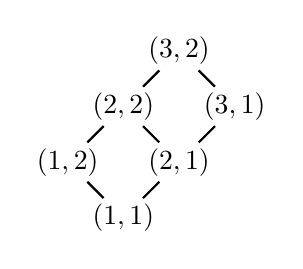
\begin{tikzpicture}
    % First, locate each of the nodes and name them
    \node (top) at (1,0) {$(3,2)$};
    \node [below left  of=top] (left)  {$(2,2)$};
    \node [below right of=top] (right) {$(3,1)$};
	\node [below left  of=left] (lleft)  {$(1,2)$};
    \node [below right of=left] (rright) {$(2,1)$};
    \node [below right of=lleft] (last) {$(1,1)$};
    % Now draw the lines:
    \draw [black,  thick, shorten <=-2pt, shorten >=-2pt] (top) -- (left);
    \draw [black, thick, shorten <=-2pt, shorten >=-2pt] (top) -- (right);
    \draw [black,  thick, shorten <=-2pt, shorten >=-2pt] (left) -- (lleft);
    \draw [black, thick, shorten <=-2pt, shorten >=-2pt] (left) -- (rright);
\draw [black, thick, shorten <=-2pt, shorten >=-2pt] (right) -- (rright);
\draw [black, thick, shorten <=-2pt, shorten >=-2pt] (last) -- (lleft);
\draw [black, thick, shorten <=-2pt, shorten >=-2pt] (last) -- (rright);
\end{tikzpicture}\end{center}

\subsubsection{Some Denotions}
\begin{itemize}
\item A Singleton is a set containing only one element.
\item $P(A) = \{B:B\subseteq A\}$
\item $A\triangle B = \{A\cup B\} \setminus \{A\cap B\}$
\item $|\R|=c=\beth_1=\aleph$
\item $A^c = \{b:b \notin A\}$
\item $\prod_{i\in I}{X_i} = \{f:I\to\bigcup_{i\in I}X_i|\forall i\in I(f(i)\in X_i)\}$
\item A pairing function is a bijection $\pi:\N\times\N\to\N$
\item The indicator function of $A\subseteq X$ is $1_A(x)=I_A(x)=\chi_A(x)=1 \iff x$ is in $A$ and equals $0$ otherwise
\end{itemize}
	
	
\end{document}